\documentclass[t]{beamer}
\usetheme{Singapore}

\usepackage{relsize}
\usepackage{xcolor}
\usepackage{array}
\usepackage{tasks}
\usepackage[nobeamer]{graphbox}

\makeatletter
  \newcommand\tinyv{\@setfontsize\tinyv{4pt}{6}} 
\makeatother

\addtobeamertemplate{navigation symbols}{}{%
	\usebeamerfont{footline}%
	\usebeamercolor[fg]{footline}%
	\hspace{1em}%
	\raisebox{\depth}{\insertframenumber/\inserttotalframenumber}
}
\setbeamercolor{footline}{fg=black}
\setbeamerfont{footline}{series=\bfseries}

\usecolortheme{rose}
\setbeamertemplate{blocks}[rounded][shadow=true]

\AtBeginSection[]
{
	\begin{frame}{Outline}
	\tableofcontents[
		sectionstyle=show/shaded,
		subsectionstyle=show/show/shaded
	]
	\end{frame}
}

\AtBeginSubsection[]
{
	\setcounter{subsection}{0}
}

\newcommand{\graphicpath}{../}

 
\title{\vspace{-2ex}\hspace{9ex} RNA SeA-SnaP \hspace{1ex}\includegraphics[scale=0.07, align=c, vshift=1ex]{\graphicpath SeA-SnaP_logo.pdf}}
\author{J. Patrick Pett\\ {\vspace{1em} \smaller CUBI, BIH}}

\date{}
 
\begin{document}

\maketitle

\frame{\frametitle{Outline} \tableofcontents}


\section{overview}

\begin{frame}
	\frametitle{pipeline overview}
	\only<1>{four main parts.}
	\only<2>{tools used in the pipeline.}
	\only<3>{helper scripts and external scripts.}
	\only<4>{example of rules:}
	\only<5>{dynamic file paths.}
	\only<6>{expansion of file paths.}
	\only<7>{choosing input files.}
	\vfill
	\centering
	\includegraphics<1>[width=0.55\textwidth]{\graphicpath pipeline_overview/pipeline_overview_2.pdf}%
	\includegraphics<2>[width=0.55\textwidth]{\graphicpath pipeline_overview/pipeline_overview_3.pdf}%
	\includegraphics<3>[width=0.55\textwidth]{\graphicpath pipeline_overview/pipeline_overview_4.pdf}%
	\includegraphics<4>[width=0.55\textwidth]{\graphicpath pipeline_overview/pipeline_overview_5.pdf}%
	\includegraphics<5>[width=0.55\textwidth]{\graphicpath pipeline_overview/pipeline_overview_6.pdf}%
	\includegraphics<6>[width=0.55\textwidth]{\graphicpath pipeline_overview/pipeline_overview_7.pdf}%
	\includegraphics<7>[width=0.55\textwidth]{\graphicpath pipeline_overview/pipeline_overview.pdf}
\end{frame}


\section{run pipeline}

\begin{frame}
\frametitle{running pipeline}
\only<1>{helper scripts to \textbf{setup pipeline}.}
\only<2>{generation of \textbf{sample summary} from input folder.}
\only<3>{generation of \textbf{covariate file} from input folder.}
\only<4>{executing snakemake pipeline.}
\vfill
\centering
\includegraphics<1>[width=0.8\textwidth]{\graphicpath run_pipeline/run_pipeline_1.pdf}%
\includegraphics<2>[width=0.8\textwidth]{\graphicpath run_pipeline/run_pipeline_2.pdf}%
\includegraphics<3>[width=0.8\textwidth]{\graphicpath run_pipeline/run_pipeline_3.pdf}%
\includegraphics<4>[width=0.8\textwidth]{\graphicpath run_pipeline/run_pipeline.pdf}
\end{frame}


\section{develop}

\subsection{pipeline}

\begin{frame}
\frametitle{develop pipeline}
rule structure:
\vfill
\centering
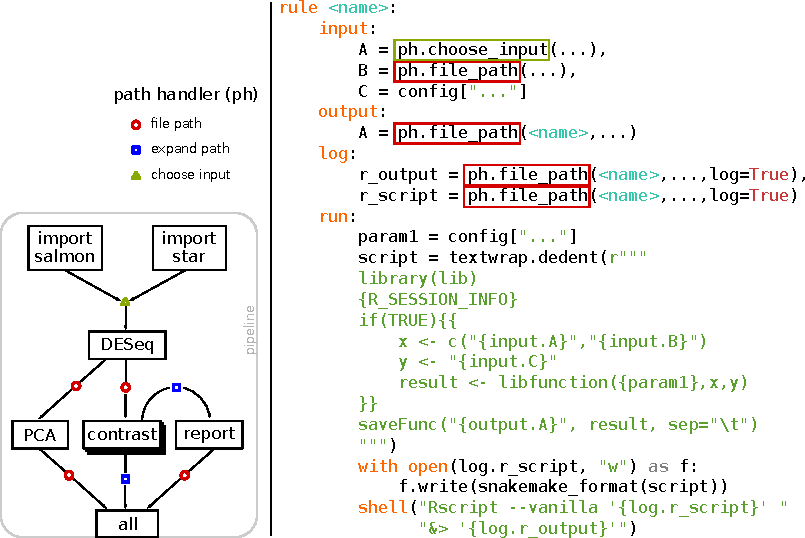
\includegraphics[width=0.9\textwidth]{\graphicpath develop/pipeline/rule_structure.pdf}%
\end{frame}

\subsection{report}

\begin{frame}
\frametitle{develop report}
develop and share \textbf{Rmd snippets} (building plan in config).
\vfill
\centering
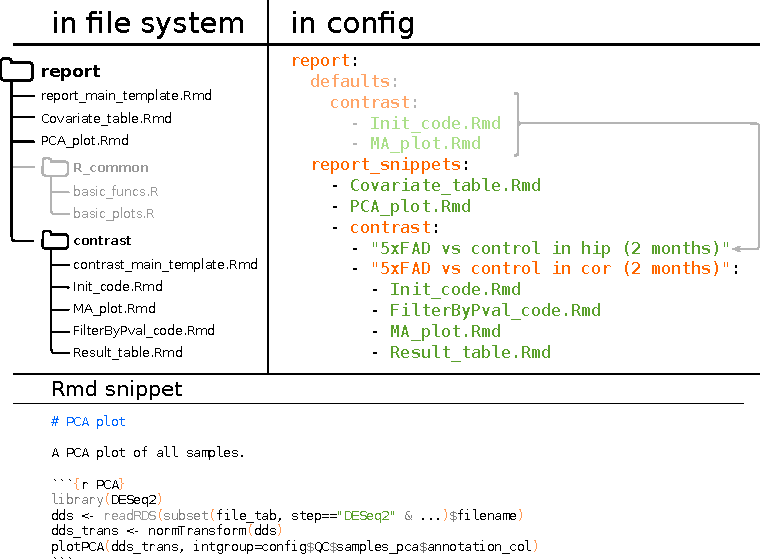
\includegraphics[width=0.8\textwidth]{\graphicpath develop/report/report_snippets.pdf}%
\end{frame}


\end{document}
